% RESULTADOS: substitua os exemplos e interprete os dados obtidos na pesquisa.
\section{Resultados e Discussão}
\label{sec:resultados-discussoes}

Apresente os resultados de acordo com os objetivos do trabalho. Explique as
tendências observadas, compare-as com a literatura e discuta limitações e
possíveis interpretações. Diferencie resultados medidos de hipóteses e expectativas.

% EXEMPLO -- gráfico de demonstração do abnTeX2. Substitua pelo seu.
A \autoref{fig_grafico} demonstra a inclusão de um gráfico em PDF.

\begin{figure}[htb]
  \centering
  \caption{Exemplo de gráfico incluído a partir de um arquivo PDF}
  \label{fig_grafico}
  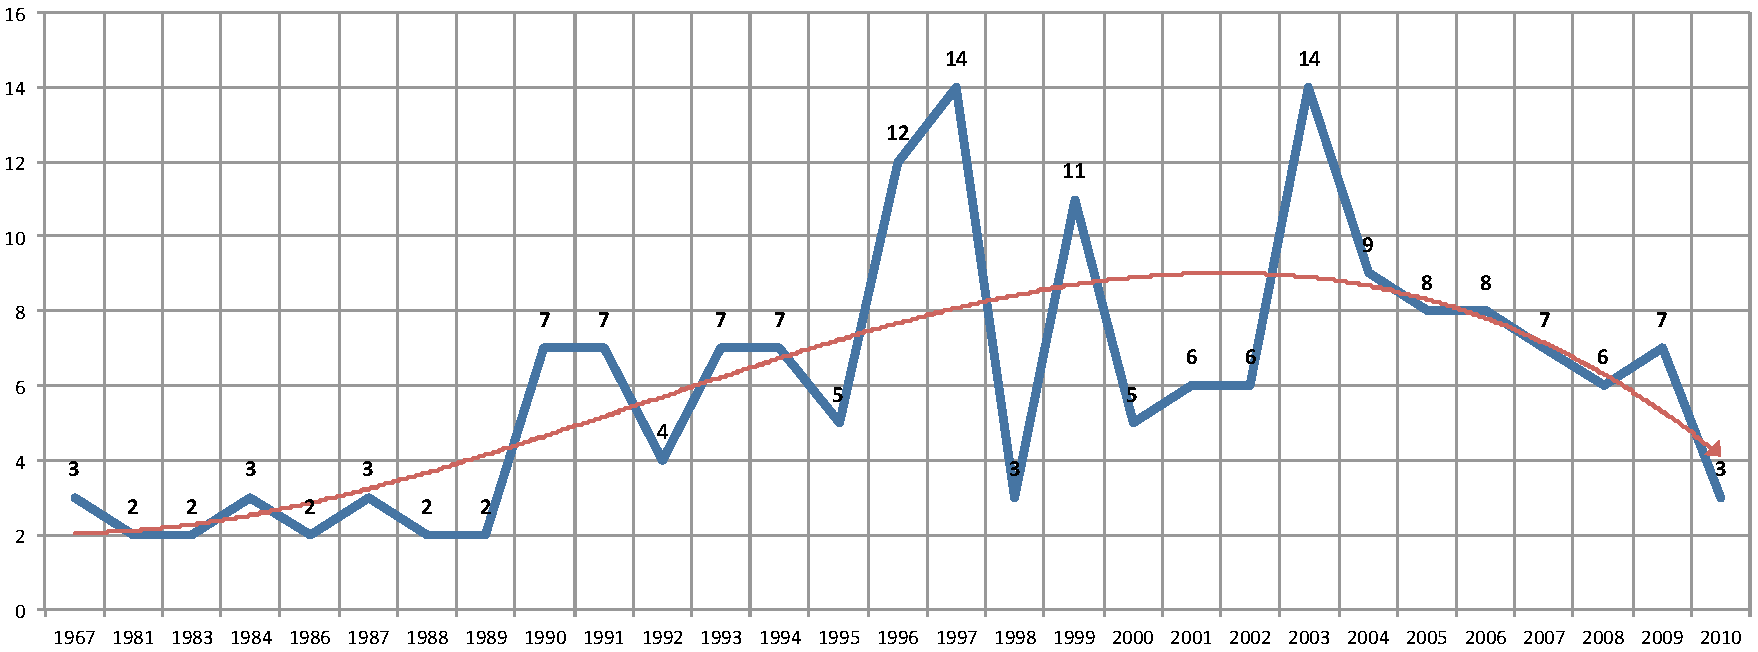
\includegraphics[width=0.7\linewidth]{imagens/abntex2-modelo-img-grafico.pdf}
  \fonte{\citeonline[p.~24]{araujo2012}.}
\end{figure}

\subsection{Equações e fórmulas}

Equações e fórmulas destacadas do parágrafo ficam centralizadas e, quando
necessário, numeradas com algarismos arábicos entre parênteses, alinhados
à direita. O ambiente \codigo{equation} faz as duas coisas; cite a equação
no texto pelo identificador, como na Equação~\ref{eq:exemplo}.

\begin{equation}
  \label{eq:exemplo}
  E = mc^{2}
\end{equation}

Se a expressão precisar ser quebrada em mais de uma linha, interrompa-a
antes do sinal de igualdade ou depois dos sinais de adição, subtração,
multiplicação e divisão.

As Figuras~\ref{fig_minipage_imagem1} e~\ref{fig_minipage_grafico2}
mostram como posicionar duas imagens lado a lado. Cada imagem tem legenda,
identificador e fonte próprios.

% Dentro de cada minipage, \linewidth corresponde à largura daquela coluna.
\begin{figure}[htb]
  \centering
  \begin{minipage}{0.46\linewidth}
    \centering
    \caption{Exemplo de imagem institucional}
    \label{fig_minipage_imagem1}
    
\includegraphics[height=2cm]{abntex-ifpi/logo_ifpi.pdf}
    \fonte{IFPI; arquivo fornecido com o modelo.}
  \end{minipage}
  \hfill
  \begin{minipage}{0.46\linewidth}
    \centering
    \caption{Exemplo de gráfico na segunda coluna}
    \label{fig_minipage_grafico2}
    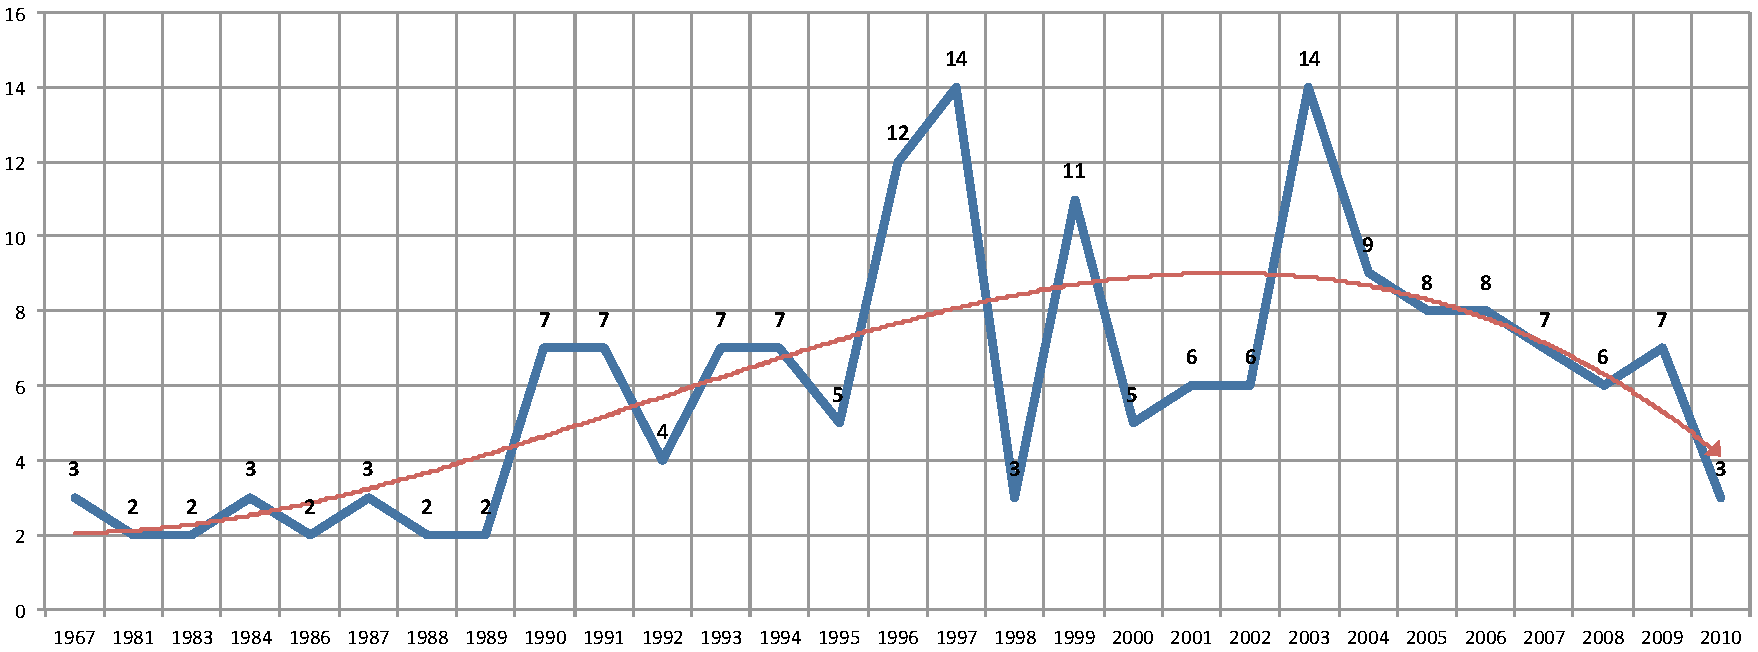
\includegraphics[width=\linewidth]{imagens/abntex2-modelo-img-grafico.pdf}
    \fonte{\citeonline[p.~24]{araujo2012}.}
  \end{minipage}
\end{figure}
